\newcommand{\sheetnum}{%
	03
}
%\setcounter{section}{\sheetnum-3}
\newcommand{\tutorialtitle}{%
    Multilayer Perceptrons and the Backpropagation algorithm 
}
\newcommand{\tutorialtitleshort}{%
	MLPs and Backprop
}
% for slides
\subtitle{\sheetnum \tutorialtitle}

\maxdeadcycles=1000 % Workaround for ! Output loop---100 consecutive dead cycles because of too many figures

% The following use of algroithms does not work well with the notes:
%
%
%
%
% instead use the following for your algorithms:
%
%\begin{figure}[!t]
%\removelatexerror
%\begin{algorithm}[H]
    % your algo here
    %\label{alg:algolabel}
    %\caption{algocaption}
%\end{algorithm}
%\end{figure}
%\begin{algorithm}
% Below is the definition for the command \removelatexerror:
\makeatletter
\newcommand{\removelatexerror}{\let\@latex@error\@gobble}
\makeatother{}

%Omit subsections from table of content
\setcounter{tocdepth}{2}

\begin{document} %%%%%%%%%%%%%%%%%%%%%%%%%%%%%%%%%%%%%%%%%%%%%%%%%%%%%%%

\sheet{\sheetnum}{\tutorialtitleshort}

\ttopic{\tutorialtitle}

\columnratio{0.2,0.8}\textbf{}
\begin{paracol}{2}
%\setlength{\columnseprule}{0.1pt}
%\setlength{\columnsep}{5em}

\begin{rightcolumn}

% notes version will ignore it
\begin{frame}
\titlepage
\end{frame}

\begin{frame}
\tableofcontents
\end{frame}

\mode<all>
\input{./mlp_feedfwd}
\mode*

\mode<article>
\section{MLPs are universal function approximators}

\begin{frame}\frametitle{\subsecname}

MLPs are universal function approximators. This means that, provided some assumptions are satisfied, they are capable of finding a function with which to map observations $\vec x$ to a their corresponding label $y_T$.

Moving forward we will focus only on \emph{scalar} values for the label $y_T$.

   \begin{block}{The universal approximation theorem by Funahashi (1989)\footnote
	{ Funahashi (1989) On the approximate realization of 
		continuous mappings by neural networks. Neur Netw, 2:183--192\\
		Hornik et al. (1989) Multilayer Feedforward Networks 
		are Universal Approximators. Neur. Netw, 2:359--366. }}
	\small
    	Let $y_T{(\vec{x})}$ be a continuous, real valued function 
    	over a compact interval $K$ and     
		\begin{equation} 
		{y}{(\vec{x}; \vec w)} = \sum_{i=1}^M \mathrm{w}_i^{21} 
		f\Big( \sum\limits_{j=1}^N \mathrm{w}_{ij}^{10} 
		  \mathrm{x}_j - \theta_i \Big)
		 \end{equation}
    	be a three-layered MLP with a non-constant, bounded, 
    	monotonously increasing and continuous function 
    	$f: \mathbb{R} \rightarrow \mathbb{R}$.\\
		\vspace{4mm}
	   \pause

		Then there exists a set of parameters 
		$M, N \in \mathbb{N}$ and $\mathrm{w}_i^{21}, 
		\mathrm{w}_{ij}^{10}, \theta_i \in \mathbb{R}$ 
		such that for every $\varepsilon > 0$:
		\begin{equation}
		\max_{\vec{x} \in K} \Big| \, y_T{(\vec{x})} - {y}{(\vec{x}; \vec w)} \,\Big| 
		\leq \varepsilon
		 \end{equation}
  \end{block}
  
\end{frame}


\mode*

\newpage

\mode<all>
\section{Ingredients for function fitting}

\begin{frame}\frametitle{\secname}

\mode<article>{
Fitting an MLP to a desired function $y_T(\vec x)$ requires the following:
}

\begin{enumerate}
\item 
\mode<article>{A cost function  with the objective to optimize it, often a minimization problem: $e(y_T, \vec x) \eqexcl \min$}
\mode<presentation>{A cost function:$e(y_T, \vec x) \eqexcl \min$}
\item A performance measure, a criterion for \emph{model selection}.
\mode<article>{Specifically, \\

the generalization \textbf{error} $E^G$ which is defined as:}	
\begin{equation} 
			E^G \quad := \quad \left<\,e\,\right>_{y_T, \vec{x}} 
			\quad = \quad \iint d \vec{x} \, dy_T \; 
				P_{(y_T, \vec{x})} \, e_{(y_T, \vec{x})}
\end{equation}

Because $P_{(y_T, \vec{x})}$ is not known, \mode<article>{we turn to the principle of empirical risk minimization (ERM).
According to ERM we can} approxomate $E^G$ by computing the empirilcal average $E^T$ using the available training data 
$\left\{\left(\vec x^{(\alpha)}, y_T^{(\alpha)}\right)\right\}, \alpha=1,\ldots,p$.
\mode<article>{The training error $E^T$ becomes:}

\begin{equation}
\text{batch training error:}\quad E^T=\sum_{\alpha=1}^{p} e^{(\alpha)}
\end{equation}
\mode<article>{
where $e^{(\alpha)}$ is the cost computed from a single observation $y(x^{(\alpha)};\vec w)$ and its corresponding label ($y_T^{(\alpha)}$). The superscript $^{(\alpha)}$ is used as an index of a specific point in the dataset.
}
\item A model with tunable parameters $\vec w$: MLP, connectionist neuron, \ldots
\item A learning algorithm\mode<article>{ for finding the set of parameters in our model that will minimize the cost function.\\
This can be done analytically (depending on some conditions) or through an iterative learning algorithm (e.g. gradient-based learning)}
\end{enumerate}

\end{frame}


\mode*

\newpage

\mode<all>
\subsection{Cost functions}
\begin{frame}\frametitle{\subsecname}
\mode<article>{
A cost function $e\tyxw$, quantifies the discrepancy between the model's prediction $y(\vec x; \vec w)$ and the label $y_T$ which $\vec x$ is assigned to.
}
Choosing a cost function accounts for 
\begin{enumerate}
\item the type of problem (i.e. regression vs. classification), 
\item how the model is penalized for different types of mistakes it can make such as:
small errors are tolerable, large errors are penalized less, etc.
\end{enumerate}
\mode<article>{
The choice of cost function has a direct effect on how the model learns. For example, we will later see in gradient-based learning how the error function can modulate how fast or slow a model learns.
}
\end{frame}

\subsubsection{Cost functions for Regression}

\begin{frame}\frametitle{\subsecname}

  \begin{tabular}{c c c}
    \parbox{4cm}{
      \[ \underbrace{\vec{x}
          \in \mathbb{R}^N
      }_{\text{feature vector}}
      \longrightarrow 
      \underbrace{y
      \in \mathbb{R}
      }_{\substack{\text{scalar}\\ \text{attribute}}}
      \]}
    & & 
    \parbox{8cm}{\footnotesize
      \begin{tabular}{l l}
	$y_T(\vec x)$: & true value of attribute \\
	$y(\vec{x}; \vec w)$: & predicted value of attribute \\
					& (e.g. by MLP)
      \end{tabular}
    }
  \end{tabular}
     \pause

  \begin{block}{individual cost $e\tyxw$}
    \begin{center} \includegraphics[width=12cm]{img/section1_fig17_v2.pdf} \end{center}
  \end{block}
\end{frame}

\begin{frame}\frametitle{Quadratic vs. linear error}

\begin{figure}[ht]
     \centering
     \savebox{\imagebox}{
	 \includegraphics[width=0.4\textwidth]{img/section1_fig17_linear}}%
     \begin{subfigure}[t]{0.45\textwidth}
         \centering
         \usebox{\imagebox}% Place largest image
         \caption{linear error}
         \label{fig:quadratic}
     \end{subfigure}
     \hfill
     \begin{subfigure}[t]{0.45\textwidth}
         \centering
         \raisebox{\dimexpr.5\ht\imagebox-.5\height}{% Raise smaller image into place
         \includegraphics[width=0.99\textwidth]{img/section1_fig17_quadratic}
         }
         \caption{qudratic error}
         \label{fig:linear}
     \end{subfigure}
     \mode<article>{
     \caption{quadratic vs. linear error}
     }
	 \label{fig:quadratic_vs_linear}
\end{figure}


\begin{equation}
e_{\text{quadratic}}\tyxw := \frac{1}{2} \Big( y_{T}(\vec x) - y(\vec x;\vec w)\Big)^{2}
\label{eq:quadratic_error}
\end{equation}

\begin{equation}
e_{\text{linear}}\tyxw := \Big| y_{T}(\vec x) - y(\vec x;\vec w)\Big|
\label{eq:linear_error}
\end{equation}
\mode<article>{
The purpose of having $\frac{1}{2}$ in \eqref{eq:quadratic_error} is for convenience for when we calculate the derivative later. 
Both the quadratic and linear cost functions are symmetric. They therefore yield the same error regardless of the sign. However, the differences between them are:
}
\end{frame}
\begin{frame}\frametitle{Quadratic vs. linear error}
\begin{table}[h]
\centering
\caption{Differences between quadratic and linear cost}
\begin{tabular}{|c|c|}
\hline
quadratic                                                                                                    & linear                                                                                                  \\ \hline \hline
\begin{tabular}[c]{@{}c@{}}larger error $\leadsto$ larger penalty\\  (sensitive to outliers)\end{tabular} & \begin{tabular}[c]{@{}c@{}}constant increase in error\\  (more stable, robust to outliers)\end{tabular} \\ \hline
\begin{tabular}[c]{@{}c@{}}converges faster\\ but slow convergence\\ for small errors\end{tabular}           & constant convergence rate                                                                               \\ \hline
differentiable everywhere                                                                                    & \begin{tabular}[c]{@{}c@{}}not differentiable at zero\\ (not a huge problem)\end{tabular}               \\ \hline
\begin{tabular}[c]{@{}c@{}}max. likelihood of\\ Gaussian variable\end{tabular}                               &                                                                                                         \\ \hline
\end{tabular}
\end{table}

\end{frame}

\newpage

\begin{frame}\frametitle{Relation between quadratic error and Gaussian labels}

\mode<article>{
\paragraph{Relation between quadratic error and Gaussian labels}\\

}

Assume labels $y_T$ are conditionally Gaussian:

\begin{equation}
P(y_T|\vec x) = \mathcal{N}(y_T|\underbrace{y(\vec x;\vec w)}_{= \mu},\sigma^2)
\label{eq:gaussian_labels}
\end{equation}

\mode<article>{
Using the quadratic cost leads to a solution that corresponds to the same solution found from maximizing the (log-)likelihood\footnote{often, the log-likelihood is maximized for computational efficiency as the log replaces the product with a sum.} of the Gaussian labels:
}
\only<1>{
%\begin{figure}[h]
     %\centering
	%\includegraphics[width=0.4\textwidth]{img/gaussian_labels}
	%\caption{Gaussian distributed labels}
	%\label{fig:gaussian_labels}
%\end{figure}

\begin{figure}[ht]
     \centering
     \savebox{\imagebox}{
	 \includegraphics[width=0.37\textwidth]{img/gaussian_labels}}%
     \begin{subfigure}[t]{0.37\textwidth}
         \centering
         \usebox{\imagebox}% Place largest image
         \caption{guassian labels}
         \label{fig:quadratic}
     \end{subfigure}
     \hspace{2mm}
     \begin{subfigure}[t]{0.37\textwidth}
         \centering
         \raisebox{\dimexpr.5\ht\imagebox-.5\height}{% Raise smaller image into place
         \includegraphics[width=0.99\textwidth]{img/qudaratic_conditional}
         }
         \caption{aggregate density}
         \label{fig:linear}
     \end{subfigure}
     \mode<article>{
     \caption{quadratic error and guassian labels}
     }
	 \label{fig:quadratic_density_gaussian}
\end{figure}
}
\only<2>{
\begin{align}
\vec w^* \in \argmin_{\vec w} \ETw 
\iff& 
\argmax_{\vec w} \underbrace{\prod_{\alpha=1}^{p} \mathcal{N}(y_T|{y(\vec x;\vec w)},\sigma^2)
}_{
\text{likelihood function } \mathcal{L(\vec w)}
}\\
&=
\argmin_{\vec w}
\underbrace{
 \lbrack - \ln \mathcal{L(\vec w)}\rbrack
 }_{\text{neg. log likelihood}}
\end{align} 
}


\end{frame}

\mode<article>{
This property makes the quadratic cost function the standard choice for regression.
}

\subsubsection{Cost functions for binary classification}

\begin{frame}\frametitle{\subsubsecname\\Deriving the cross entropy cost function for binary classification}

\mode<article>{
\paragraph{Deriving the cross entropy cost function for binary classification}\\
}

\begin{itemize}
\item[]\underline{Data}:\\

\begin{equation}
\Big\{ \left( \vec x^{(\alpha)}, y_T^{(\alpha)} \right) \Big \}_{\alpha=1}^{p}
\end{equation}

with 
$$
\vec x^{(\alpha)} \in \R^N\;\;,\;\; y_T^{(\alpha)} \in \{{\color{red}0}, {\color{blue}1}\}.
$$

generated by
\begin{equation}
\left( \vec x^{(\alpha)}, y_T^{(\alpha)} \right) \stackrel{\iid}{\sim} P_{\text{data}}(\vec x, y)
\end{equation}

\pause

\item[]\underline{Model}:\\

MLP, scalar output \mode<article>{interpreted as probability that $y(\vec x; \vec w)=1$. In other words the probability of $\vec x$ belonging to class '1' (the positive class):}

\begin{equation}
y(\vec x;\vec w) =: P_{\text{model}} ({\color{blue}y=1}|\vec x;\vec w) \;\; \text{and} \;\; P_{\text{model}} ({\color{red}y=0}|\vec x; \vec w) = 1-y(\vec x;\vec w)
\end{equation}

for the \textcolor{blue}``positive'' and ``negative''/``other'' class respectively.

\end{itemize}

\end{frame}

\begin{frame}\frametitle{Cost function derivation via minimization of \\the Kullback-Leibler divergence}

\mode<article>{
\paragraph{The Kullback-Leibler divergence }\\

}

$\dkl(P||Q)$ is a measure of how much a probability distribution $P$ differs from another distribution $Q$.

Properties of the KL-divergence:

\begin{itemize}
\item $\dkl = 0$ iff. both distribution are \emph{identical}.
\item Otherwise $\dkl > 0$.
\item Does not qualify as a metric because it is not symmetric. For different distributions P and Q: $\dkl(P_||Q) \ne \dkl(Q||P)$
\end{itemize}

\end{frame}

\begin{frame}\frametitle{Cost function derivation via minimization of the Kullback-Leibler divergence}
 
From KL-divergence to binary cross entropy loss:
\only<1>{

\begin{align}
\dkl\left(\, P_{\text{data}}(\vec x, ) \,||\, P_{\text{model}}(\vec x, y) \,\right)
= \iint d \vec x dy P_{\text{data}}(\vec x, y)
\ln 
\left( 
\frac{P_{\text{data}}(\vec x, y)}{P_{\text{model}}(\vec x, y)}
\right)
\end{align}

\mode<article>{
Integrating w.r.t. $y$ $\corresponds$ sum over the set of all possible values for $y$, which is $\{0,1\}$ in this case:
}
}
\definecolor{darkgreen}{rgb}{0,0.6,0}
\begin{align}
\only<1,2>{
\dkl&\left(\, P_{\text{data}}(\vec x, y) \,||\, P_{\text{model}}(\vec x, y) \,\right)\\
&= \int_{\R^N} d \vec x \sum_{y \in \{0,1\}} P_{\text{data}}(\vec x, y) \ln 
\left( 
\frac{P_{\text{data}}(\vec x, y)}{P_{\text{model}}(\vec x, y)}
\right)\\
}
\only<1,2>{
&= \int_{\R^N} d \vec x \sum_{y \in \{0,1\}} 
	\underbrace{
		P_{\text{data}}(\vec x)P_{\text{data}}(y | \vec x)
	}_{
		\substack{
		=P_{\text{data}}(\vec x, y)\\(\text{Bayes' rule})
		}
	}
	\ln 
	\left( 
		\frac{ P_{\text{data}}(\vec x)P_{\text{data}}(y | \vec x) }
		{
		\smash{
			\underbrace{
				P_{\hcancel[red]{\text{model}}}(\vec x)
				}_{
				\substack{
					\color{red}\text{discriminative model}\\
					\color{red}\text{not a generative model}\\
					\color{red}\text{replace with }
					{\color{cyan} P_{\text{data}}(\vec x)}
				}%substack
			}%underbrace
			\hspace{-5mm}
			P_{\text{model}}(y | \vec x)
		}%smash
		}%frac(lower)
	\right) \\
}
\only<2,3,4>{
&= \int_{\R^N} d \vec x \sum_{y \in \{0,1\}} 
	\underbrace{
		\color{darkgreen}
		P_{\text{data}}(\vec x)
	}_{\text{indep. of } y}
	P_{\text{data}}(y | \vec x)
	\ln 
	\left( 
	\frac{
		{ \color{cyan} P_{\text{data}}(\vec x) }
		{ \color{violet} P_{\text{data}}(y | \vec x) }
	}
	{
		{ \color{cyan} P_{\text{data}}(\vec x) }
		{ \color{brown} P_{\text{model}}(y | \vec x) }
	}%frac(lower)
	\right) \\
}
\only<3,4>{
&= \underbrace{
	\int_{\R^N} d \vec x \,
	{ \color{darkgreen} P_{\text{data}}(\vec x) }
	\sum_{y \in \{0,1\}}
	P_{\text{data}}(y | \vec x)
	\ln 
	\lbrack { \color{violet} P_{\text{data}}(y | \vec x) } \rbrack
	}_{\text{indep. of model parameters } \vec w} \\
	&\qquad- \int_{\R^N} d \vec x \,
		{ \color{darkgreen} P_{\text{data}}(\vec x) }
		\underbrace{
			\sum_{y \in \{0,1\}}
			P_{\text{data}}(y | \vec x)
			\ln
			\lbrack {\color{brown} P_{\text{model}}(y | \vec x) } \rbrack
		}_{
		\substack{
		\text{\textbf{cross entropy} between } \\
		\text{data \& model distributions given }\vec x}
		}
}
\end{align}

\mode<presentation>{
\only<4>{
Apply ERM on the \textbf{cross entropy} term.
}
}

\end{frame}

\begin{frame}\frametitle{ERM}

\mode<article>{
ERM for computing cross entropy loss using the training data:
}
\mode<presentation>{
\vspace{-5mm}
}

\begin{align}
\onslide<1->{
\ETw &= \frac{1}{p} \sum_{\alpha=1}^{p} - \bigg( \;
	\sum_{y\in\{{\color{red}0},{\color{blue}1}\}} P_{\text{data}}(y | \vec x^{(\alpha)})
	 \ln \lbrack P_{\text{model}}(y | \vec x^{(\alpha)}) \rbrack
	 \;\bigg)\\
	 &= \frac{1}{p} \sum_{\alpha=1}^{p} - \bigg( \;
	P_{\text{data}}({\color{blue}y=1} | \vec x^{(\alpha)})
	 \ln \lbrack P_{\text{model}}({\color{blue}y=1} | \vec x^{(\alpha)}) \rbrack \\
	 &\qquad\qquad\qquad+
	 P_{\text{data}}({\color{red}y=0} | \vec x^{(\alpha)})
	 \ln \lbrack P_{\text{model}}({\color{red}y=0} | \vec x^{(\alpha)}) \rbrack 
	  \;\bigg)\\
}
\onslide<2->{
	 &= \frac{1}{p} \sum_{\alpha=1}^{p} - \bigg( \;
		{\color{blue}y_T^{(\alpha)}} \cdot
	 \ln \lbrack {\color{blue}y(\vec x^{(\alpha)};\vec w)} \rbrack
	 + ( {\color{red}1-y_T^{(\alpha)}} ) \cdot
	 \ln \lbrack {\color{red}1-y(\vec x^{(\alpha)};\vec w)} \rbrack
	 \;\bigg)\\
}
\onslide<3->{
	 &= \frac{1}{p} \sum_{\alpha=1}^{p} \bigg( -
		{\color{blue}y_T^{(\alpha)}} \cdot
	 \ln \lbrack {\color{blue}y(\vec x^{(\alpha)};\vec w)} \rbrack
	 - ( {\color{red}1-y_T^{(\alpha)}} ) \cdot
	 \ln \lbrack {\color{red}1-y(\vec x^{(\alpha)};\vec w)} \rbrack  \;\bigg) \\
	 &= \frac{1}{p} \sum_{\alpha=1}^{p} e\tyxwalpha
}
\end{align}

Extendable to multi-class cross entropy alongside \emph{softmax} normalization.

\end{frame}

\begin{frame}
    
{\renewcommand{\arraystretch}{1.2} %<- control vertical spacing
\begin{table}[h!]
\caption{Cost functions \& output layers}\slidesonly{\vspace{-5mm}}
\resizebox{\textwidth}{!}{%
\begin{tabular}{|l|c|c|l|}
\hline
task 
&  
\begin{tabular}[c]{@{}c@{}}\multicolumn{1}{c}
~\\[-5mm]
data\\
$\big\{ \vec x^{(\alpha)}, y_T^{(\alpha)} \big\}_{\alpha=1}^{p}$\\[2mm]
\end{tabular}
& output layer 
& \begin{tabular}[c]{@{}c@{}}
    cost function\\ 
    $e := e\tyxw$\end{tabular} \\ 
\hline \hline
scalar regression 
& 
$y_{T} \in \R$
& \begin{tabular}[c]{@{}l@{}}linear\\ $y = {\vec w^{LL-1}}^{\top} \vec s^{L-1}$\end{tabular} 
& \begin{tabular}[c]{@{}c@{}}quadratic error\\
$e = \frac{1}{2} \big( y_{T} - y\big)^{2}$\end{tabular} 
\\ \hline
\begin{tabular}[c]{@{}l@{}}multivariate linear \\ regression\end{tabular} 
&  
$\vec y_{T} \in \R^{M}$
& \begin{tabular}[c]{@{}l@{}}linear\\ $y_{k} = {\vec w_{k}^{LL-1}}^{\top} \vec s^{L-1}$\end{tabular} 
& \begin{tabular}[c]{@{}c@{}}squared Euclidean \\ distance\\ 
$e = \frac{1}{2} \lVert \vec y_{T} - \vec y \rVert^{2}_{2}$
\end{tabular} \\ 
\hline
\begin{tabular}[c]{@{}l@{}}binary \\ classification\end{tabular} 
&  $y_{T} \in \{0,1\}, \{-1,1\}$
&
\begin{tabular}[c]{@{}c@{}}logistic sigmoid\\ 
$y = \frac{1}{1+exp(-h_{1}^{L})}$\\
or $y = \tanh(h_{1}^{L})$
\end{tabular} 
& \begin{tabular}[c]{@{}l@{}}cross entropy\\ 
$
e = \kern-.5ex
- y_T
\ln \lbrack y \rbrack \quad$\\
$
\;
-\kern-.2ex ( 1\kern-.5ex-\kern-.5exy_T )
\ln \lbrack 1\kern-.5ex-\kern-.5exy \rbrack
$
\end{tabular} \\ 
\hline
\begin{tabular}[c]{@{}l@{}}multi-class \\ classification\\ with $M$ classes\end{tabular} 
&  
\begin{tabular}[c]{@{}c@{}}
$y_{T} \in \{0,1\}^{M}$\\
1-out-of-M encoding/\\
1-hot-encoding\\
e.g. $y_{T}=(0,0,1,0)^{\top}$\\ $\corresponds$ class 3 out of 4
\end{tabular}
& \begin{tabular}[c]{@{}c@{}}softmax\\ 
$y_{k} = \frac{exp(h_{k}^{L})}{\sum_{k=1}^{M} exp(h_{k}^{L})}$\\[5mm]
$\Rightarrow \sum_{k=1}^{M} y_{k} = 1$
\end{tabular}
& \begin{tabular}[c]{@{}c@{}}cross entropy\\(multi-class case)\\ 
$
e = \kern-.3ex
-\kern-.2ex\sum_{k=1}^{M} {y_T}_{k} $\\
$\;\;\cdot 
%$\cdot
\ln \lbrack y_{k}\big(\vec x; \vec w\big) \rbrack
$
\end{tabular} \\
\hline
\end{tabular}
}
\end{table}
} % arraystretch

\end{frame}

\mode*

\clearpage

\mode<all>
\section{Gradient-based learning}

\begin{frame}\frametitle{\secname}


\end{frame}


\mode*

\clearpage

\mode<all>
\section{The backpropagation algorithm}

\begin{frame}\frametitle{\secname}

The Backpropagation algorithm is a method for computing gradients by using the chain rule efficiently.

\end{frame}


\definecolor{darkgreen}{rgb}{0,0.6,0}
\definecolor{darkcyan}{rgb}{0,0.5,0.5}
\definecolor{darkyellow}{rgb}{0.5,0.5,0}
\definecolor{mangenta}{rgb}{1,0,1}
% -----------------------------------------------------------------------------
\begin{frame} \frametitle{Gradients in neural networks}
	\begin{equation*}
	\textcolor{orange}{	\frac{\partial y(\vec{x}; \vec{w})}{
			\partial \mathrm{w}_{ij}^{v'v}}}
	\end{equation*}

	\begin{center} \includegraphics[height=3.5cm]{img/section1_fig20.pdf} \end{center}

		%~ \begin{minipage}{3.5cm}
	\hspace{0.9cm} \tiny Bias node included in the parents.
		%~ \end{minipage}
	\vspace{0.3cm}\\
	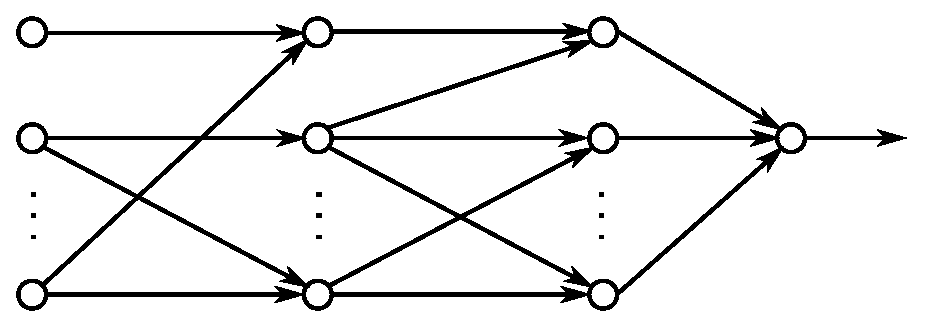
\includegraphics[width=4cm]{img/MLP_horizontal.eps}
	%\hfill{\tiny see blackboard for derivation}
\end{frame}

% -----------------------------------------------------------------------------
\begin{frame} \frametitle{Gradients in neural networks} 

	\placeimage{9.5}{1}{img/section1_fig20_mini_multicolor.pdf}{width=4.8cm}	
	\vspace{9mm}
	%How do the weights $w_{ij}^{v'v}$ of hidden units $S_i^{v'}$
   	%contribute to the error?
	\begin{block}{Solution: smart application of the chain rule}
		\begin{eqnarray*}
			{\color{darkgreen}h_i^{v'}} 
	   			&=& \kern-2ex\smallsum{(\mu,k) \in P(v',i)}{} \kern-2ex
	   			w_{ik}^{v'\mu}\;  f_k^\mu\big( {\color{teal} h_k^\mu} \big)
	   		\\[4mm]
			\frac{\partial y(\vec{x}; \vec{w})}{\partial \mathrm{w}_{ij}^{v'v}}
				&=& \underbrace{\frac{\partial y(\vec{x}; \vec{w})}
					{{\color{darkgreen}\partial h_i^{v'}}} }_{ 
						\substack{\coloneqq\;{\color{red}\delta_i^{v'}} \\
						\text{``local error''} \\
						\text{at neuron} \\
						(v', i)}
					}
				  \cdot 
				  \underbrace{\frac{{\color{darkgreen}\partial h_i^{v'}}}
				  	{\partial \mathrm{w}_{ij}^{v'v}}}_{
						\substack{=\;f_j^v({\color{teal} h_j^v}) \\
						\text{activity} \\
						\text{of neuron} \\
						(v, j)}}
		\end{eqnarray*}
	\end{block}
\end{frame}

% -----------------------------------------------------------------------------
\begin{frame} \frametitle{Gradients in neural networks}
	\only<1,2>{\placeimage{9.5}{1}{img/section1_fig20_mini_multicolor.pdf}{width=4.8cm}}
	\only<3->{\placeimage{9.5}{1}{img/section1_fig20_mini_back_multicolor.pdf}{width=4.8cm}}
	
	\vspace{11mm}
	\begin{enumerate}
		\item {\textbf forward propagation}: calculate activities 
				$f_i^{v'}({\color{darkgreen}h_i^{v'}})$
				{\small(parents $\rightarrow$ children)}
				$$	
					{
					%\color{darkgreen}
					h_j^0
					} 
						\;:=\; \mathrm{x}_j \,, 
					\quad 
					{\color{darkgreen}h_i^{v'}}
		   			\,= \kern-2ex\smallsum{(\mu,k) \in P(v',\,i)}{} \kern-2ex
	   			w_{ik}^{v'\mu}\;  f_k^\mu\big( {\color{teal} h_k^\mu} \big) \,,
					\quad
					y(\vec{x}; \vec{w})\,=\, f_1^L({\color{blue}h_1^L})
				$$\\[-2mm]
	\only<1>{	
		\mode<presentation>{
		\begin{center}
		\vspace{2mm}
		\includegraphics[height=4cm]{img/section1_fig14}
		\end{center}
		}
	}
	\only<2>{	
		\mode<presentation>{
		\begin{center}
		\vspace{2mm}
		\includegraphics[height=4cm]{img/section1_fig14_fwd}
		\end{center}
		}
	}
	\only<3->{
		\item {\textbf backpropagation}: calculate ``local errors'' 
				$\color{red}\delta_i^{v'}$
				{\small(children $\rightarrow$ parents)}
				\vspace{-1mm}
				%~ \begin{eqnarray*} 
				%~ \end{eqnarray*}
				\begin{eqnarray*} 
				{\color{red} \delta_1^L}
				&=& \frac{\partial y(\vec{x}; \vec{w})} {{\color{blue}\partial h_1^{L}}}
					= [f_1^{L}]'({\color{blue} h_1^{L}})
							%\;\;\text{for}\;v'=L
							\\
					{\color{red}\delta_i^{v'}} 
					\only<3>{
						&=&  \frac{\partial y(\vec x; \vec w)}{\partial h^{v'}_{i}}
						\qquad \text{local error at neuron }(v', i)\\
						}
					\only<4->{
						&=&  \kern-3ex\sum\limits_{(v''\hspace{-1mm},\,k) \in C(v',\,i)}
						\underbrace{
							\smallfrac{\partial y(\vec{x}; \vec{w})}
								{{\color{blue}\partial  h_k^{v''}}}
							}_{{\color{red}\delta_k^{v''}}} 
						\;\kern1.5ex\cdot \kern-2.5ex\;
						\underbrace{\smallfrac
								{{\color{blue}\partial h_k^{v''}} }
								{{\color{darkgreen}\partial h_i^{v'}}}
							}_{\mathrm{w}_{ki}^{v''v'} \kern-.5ex\cdot\kern.5ex
								[f_i^{v'}]'({\color{darkgreen}h_i^{v'}}) } %\,,
					\kern-3ex=\;\;\; %\underbrace{
							[f_i^{v'}]'({\color{darkgreen}h_i^{v'}}) 
							\kern-3ex\sum_{(v''\hspace{-1mm},\,k) \in C(v',\,i)}\kern-3ex
							{\color{red}\delta_k^{v''}} 
							\mathrm{w}_{ki}^{v'' v'} 
						}
						%}_{{\color{red} \delta_i^L}\;=\;
						%	[f_i^{L}]'({\color{darkgreen} h_i^{L}})
						%	\;\;\text{for}\;v'=L}
				\end{eqnarray*}
		}
		\only<5->{
		\vspace{-1mm}
		\item {\textbf weight update}: using activities and local errors
			$$
				\mathrm{w}_{ij}^{v'v}
				\quad \leftarrow \quad 
				\mathrm{w}_{ij}^{v'v} - \eta \cdot
				\smallfrac{\partial e}{\partial\mathrm{w}_{ij}^{v'v}}
				\quad=\quad \mathrm{w}_{ij}^{v'v} - \eta \cdot
				\smallfrac{\partial e}{\partial y(\vec{x}; \vec{w})} \cdot
				\only<5>{
				\smallfrac{\partial y(\vec{x}; \vec{w})}{\partial\mathrm{w}_{ij}^{v'v}}\hspace{8.5mm}
				}
				\only<6>{
				{\color{red} \delta_i^{v'}} \kern-.5ex\cdot
			   			f_j^v( {\color{darkgreen}h_j^v} )
			   	}
			$$
			}
	\end{enumerate}
	%{\scriptsize
	%Computational complexity: $O(n)$, $n$: number of weights \& thresholds}
\end{frame}

% -----------------------------------------------------------------------------
\definecolor{forward}{rgb}{0,0.7,0}
\definecolor{backward}{rgb}{0.8,0,0}
\begin{frame} \frametitle{Summary of the backpropagation for gradient descent}
	\only<1>{
		\placeimage{10.75}{5.5}{img/MLP_forward.pdf}{width=3.75cm}
		\placeimage{10.75}{8.7}{img/MLP_backward.pdf}{width=3.75cm}
	} \only<2> {
		%\begin{minipage}{4}(11.5,5)
			%{\color{blue}
				%\footnotesize
				%\begin{center}
					%computational and 
					%memory complexity \\[2mm]
					%{\color{red}
						%$\mathcal{O}(n)$, %\quad
					%} \\[2mm]
					%$n$: number of weights
					%i.e.~{\em linear} in the 
					%number of weights
				%\end{center}
			%}
		%\end{minipage}
	}
	
	%\begin{algorithm}[H] 
		%\scriptsize
		\footnotesize
		\DontPrintSemicolon
		initialization of weights and thresholds \\
		\While{stopping criterion not met}{
			$\text{gradient}_{ij}^{v'v} := 0 
					\,, \quad \forall w_{ij}^{v'v}$ \\
			\For{$\alpha \in \{1,\ldots,p\}$}{
				${\color{forward}h_i^0} 
					:= x_i^{(\alpha)} \,, \quad \forall i$ 
				\qquad\qquad // {\color{forward}forward propagation}\\
				\For{$v' \in \{1,\ldots,L\}$}{
					%~ ${\color{forward} h_i^{v'}} 
						%~ := \sum\limits_{\scriptscriptstyle
							%~ (v',i) \in C(v,j)} w_{ij}^{v'v} 
							${\color{forward}h_i^{v'}}
		   			\;\;=\;\; \kern-2ex\smallsum{(\mu,k) \in P(v',i)}{} \kern-2ex
	   			w_{ik}^{v'\mu}\;  \underbrace{f_k^\mu\big( {\color{forward} h_k^\mu} \big) 
								%~ \underbrace{f_j^v({\color{forward} h_j^{v}})
								}_{\kern-2exx_k^{(\alpha)} \;\text{if}\; 
									v'=1\kern-2ex } \,,
							\quad \forall i$
					\vspace{-1.5mm}
				}
				${\color{backward} \delta_1^L} 
					:= [f_1^L]'({\color{forward}h_1^L}) $%\,, \quad \forall i$ 
				\qquad // {\color{backward}backward propagation}\\
				\For{$v' \in \{L-1,\ldots,1\}$} {
					${\color{backward}\delta_i^{v'}} 
						:= [f_{i}^{v'}]'({\color{forward}h_i^{v'}}) 
						\kern-1ex\sum\limits_{(\mu,k) \in C(v',i)}\kern-1ex
						{\color{backward} \delta_k^{\mu}} 
						\, w_{ki}^{\mu v'} \;,
						\quad \forall i$
					\vspace{-2.5mm}
				}
				$\text{gradient}_{ij}^{v'v} := \text{gradient}_{ij}^{v'v}
						+ \frac{\partial e^{(\alpha)}}{\partial y(\vec x; \vec w)}
						 \, {\color{backward}\delta_i^{v'}} 
						 \, f_j^v({\color{forward}h_j^v})
						 \,, \quad \forall w_{ij}^{v'v}$
				\hspace{11mm} // sum
			}
			$\text{gradient}_{ij}^{v'v} := \frac{1}{p} \text{gradient}_{ij}^{v'v}$\\
			% $w_{ij}^{v'v} := w_{ij}^{v'v} - \frac{\hat \eta}{p}
			 $w_{ij}^{v'v} := w_{ij}^{v'v} - \eta
					\, \text{gradient}_{ij}^{v'v} 
					\,, \quad \forall w_{ij}^{v'v}	$
			\hspace{15mm} // gradient descent step
					\vspace{-1.5mm}
		}
		%\caption{Backpropagation in feedforward networks}
	%\end{algorithm}
\end{frame}

\mode*

\clearpage

\mode<all>
\input{./mlp_symmetries}
\mode*

\end{rightcolumn}
\end{paracol}

\end{document}
